\documentclass[a4paper,12pt,article,firamath]{nsi}
\titre{DM arbres binaires}
\classe{NSI2}
\begin{document}
\maketitle
\section*{\'Etude théorique}

    \begin{encadrecolore}{Rappel}{UGLiRed}
        Soit $n$ un entier naturel, on a $$\sum_{k=0}^{k=n}2^k = 2^{n+1}-1$$
        C'est à dire que
        $$1+2+4+\ldots+2^n=2^{n+1}-1$$
        Ou encore $$(\underbrace{1\ldots 1}_{n\text{ bits}})_2=2^{n+1}-1$$
    \end{encadrecolore}

    On considère un arbre binaire \textbf{parfait} et on numérote ses n\oe uds de la manière suivante:
    \begin{itemize}
        \item la racine a le numéro 1;
        \item les 2 n\oe uds de hauteur 1 sont numérotés de gauche à droite respectivement 2 et 3;
        \item les 4 n\oe uds de hauteur 2 sont numérotés de gauche à droite respectivement 4, 5, 6 et 7;
        \item et ainsi de suite.
    \end{itemize}

    \begin{enumerate}
        \item Compléter la numération de cet arbre de hauteur 4.

        \begin{center}
            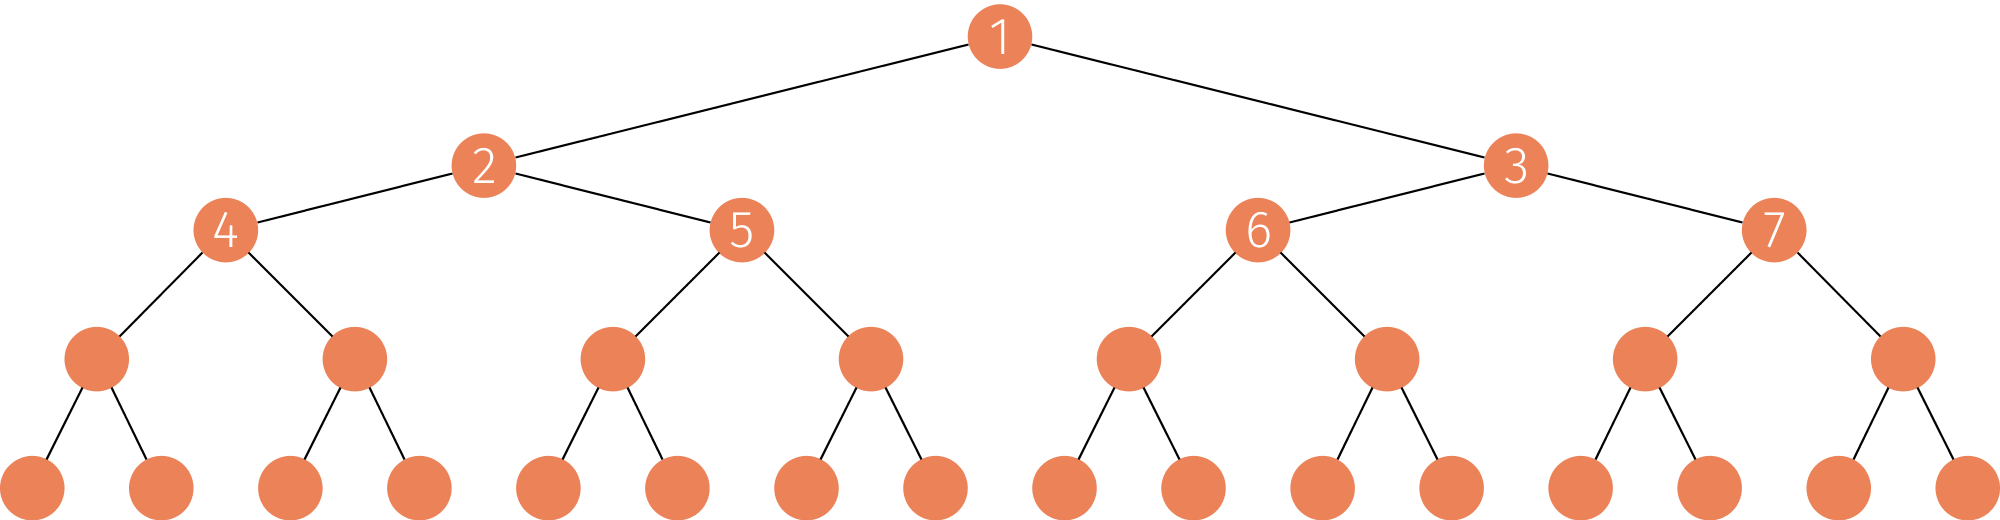
\includegraphics[width=\linewidth]{img/arbre3}
        \end{center}
        \item On considère un arbre binaire \textbf{parfait} de hauteur $h\in \N$.\\
        Soit $p$ un entier naturel inférieur ou égal à $h$, combien y a-t-il de n\oe uds de hauteur $p$ dans l'arbre ? \\
        Comment prouver ce résultat ?
        \item On considère un n\oe ud $\mathcal{N}$ de hauteur $p$ et on note $i\left(\mathcal{N}\right)$ son numéro.\\
        Que vaut $i\left(\mathcal{N}\right)$ au minimum ? Au maximum ?\\
        Comment prouver ces affirmations ? On pourra utiliser le rappel.
        \item Quels sont les numéros du fils gauche de $\mathcal{N}$ et du fils droit de $\mathcal{N}$ ? Comment prouver ces résultats ?
        \item Soit un n\oe ud numéroté $k\geqslant 2$, quel est le numéro de son père ?
    \end{enumerate}

    \section*{Implémentation}

    On décide de représenter un arbre parfait de hauteur $h$ avec une liste de la bonne taille, l'élément d'indice 0 ne servant pas, celui d'indice 1 contenant la racine \textit{et c\ae tera}.\\

    \begin{enumerate}
        \item \'Ecrire la fonction \texttt{create\_perfect\_tree} qui:
        \begin{itemize}
            \item en entrée prend un \mintinline{python}{int} \texttt{h};
            \item en sortie renvoie une valeur de type \mintinline{python}{list}, avec les numéros des n\oe uds aux indices correspondants.
        \end{itemize}
        Par exemple \mintinline{python}{create_perfect_tree(3)} renverra \mintinline{python}{[None, 1, 2, 3, 4, 5, 6, 7]}
        \item Créer les fonctions \mintinline{python}{left} et \mintinline{python}{right} qui
        \begin{itemize}
            \item en entrée prennent un \mintinline{python}{int i};
            \item renvoient l'indice du fils gauche (respectivement du fils droit) de \mintinline{python}{i}.
        \end{itemize}
        À ce niveau on ne se soucie pas des \mintinline{python}{IndexError}.
        \item Implémenter la fonction \mintinline{python}{prefix} qui devra réaliser l'affichage des n\oe uds selon un parcours préfixe. (Conseil, passer la liste et l'indice en paramètres et procéder récursivement, les cas d'arrêt se produisant si on voit qu'on va obtenir une \mintinline{python}{IndexError}).
        \item Faire de même avec les fonctions \mintinline{python}{infix} et \mintinline{python}{postfix}.
    \end{enumerate}
\end{document}